\chapter{Adopting Agile Methodologies}
\label{ch:agile-solutions}

Djøf Trade Union addressed their challenges by adopting Scrum practices that introduced structure and transparency. The Scrum framework emphasizes empiricism through transparency, inspection, and adaptation \textit{\parencite{schwaber2020scrum}}. Research demonstrates that successful adoption requires adapting frameworks to organizational realities \textit{\parencite{verwijs2021scrum}}. This chapter examines how they implemented Scrum to deliver value more consistently.

\section{Establishing Product Backlog Refinement}
\label{sec:refinement-process}

Structured refinement sessions changed how work reached the development team. Before refinement, tasks arrived without analysis of feasibility or value. The refinement process gave the team a mechanism to break down initiatives and identify issues early. Product Backlog refinement is an ongoing activity where teams add detail, estimates, and order to items \textit{\parencite{schwaber2020scrum}}.

Ahmed described how refinement works: before starting any project, the team breaks down epics into user stories \textbf{(Transcript: 00:05:30)}. The team takes business needs from stakeholders and decomposes them into manageable tasks, allowing incremental delivery. When business preparation is thorough and each story has clear purpose, projects succeed \textbf{(Transcript: 00:06:00)}.

This practice addressed the legacy system problem. The checkbox task should never have reached developers without verifying legal approval first. Refinement created gatekeeping that prevents such situations. They now question assumptions, identify dependencies, and validate feasibility during refinement rather than discovering blockers later. The process also improved transparency for stakeholders: when epics break into many user stories, stakeholders gain realistic insight into complexity.

\begin{figure}[h]
\centering
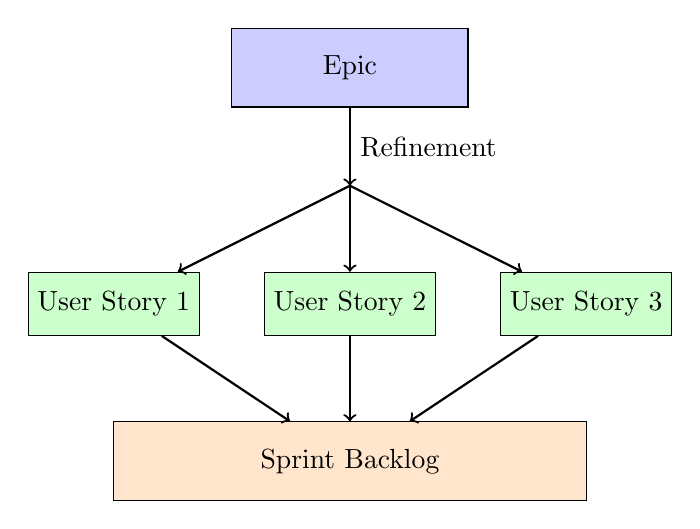
\begin{tikzpicture}
    % Epic box
    \node[draw, rectangle, fill=blue!20, minimum width=3cm, minimum height=1cm] (epic) at (0,0) {Epic};

    % Arrow down
    \draw[->, thick] (epic) -- (0,-1.5) node[midway, right] {Refinement};

    % User stories
    \node[draw, rectangle, fill=green!20, minimum width=2cm, minimum height=0.8cm] (us1) at (-3,-3) {User Story 1};
    \node[draw, rectangle, fill=green!20, minimum width=2cm, minimum height=0.8cm] (us2) at (0,-3) {User Story 2};
    \node[draw, rectangle, fill=green!20, minimum width=2cm, minimum height=0.8cm] (us3) at (3,-3) {User Story 3};

    % Arrows to user stories
    \draw[->, thick] (0,-1.5) -- (us1);
    \draw[->, thick] (0,-1.5) -- (us2);
    \draw[->, thick] (0,-1.5) -- (us3);

    % Sprint backlog
    \node[draw, rectangle, fill=orange!20, minimum width=6cm, minimum height=1cm] (backlog) at (0,-5) {Sprint Backlog};

    % Arrows to backlog
    \draw[->, thick] (us1) -- (backlog);
    \draw[->, thick] (us2) -- (backlog);
    \draw[->, thick] (us3) -- (backlog);

\end{tikzpicture}
\caption{Product Backlog Refinement Process: epics are decomposed into manageable user stories through collaborative refinement sessions.}
\label{fig:refinement-workflow}
\end{figure}


\section{Introducing Scrum Roles and Sprint Structure}
\label{sec:scrum-roles-sprints}

Defined Scrum roles brought accountability and clarity. Scrum defines three accountabilities: Product Owner, Scrum Master, and Developers \textit{\parencite{schwaber2020scrum}}. The Product Owner prioritizes the backlog in collaboration with the business, evaluating which work delivers most value while considering technical dependencies \textbf{(Transcript: 00:14:52)}. This resolved the situation where everything seemed equally urgent. The Scrum Master maintains the process and removes obstacles \textbf{(Transcript: 00:16:52)}.

They adopted two week sprints after experimenting with different lengths. Three week sprints proved too long, while one week sprints were too short to deliver meaningful increments \textbf{(Transcript: 00:14:07)}. The two week cadence provided sufficient time to complete user stories while maintaining rapid feedback cycles.

The team adapted Scrum pragmatically: they dropped story points because stakeholders misinterpreted them as time commitments \textit{\parencite{russo2021agile}} \textbf{(Transcript: 00:08:58)}. They occasionally skip retrospectives when sprints lack meaningful progress \textbf{(Transcript: 00:09:59)}, demonstrating focus on outcomes over ceremony.

Sprint reviews provide regular checkpoints to evaluate success and learn from failures \textbf{(Transcript: 00:06:48)}. Retrospectives offer space to refine how the team works together. These ceremonies established inspection and adaptation cycles absent previously.

\section{Building Collaboration and Transparency}
\label{sec:collaboration-transparency}

The visible backlog allowed stakeholders to see work in progress and understand capacity constraints. When stakeholders wanted new features, they could observe how requests fit into existing priorities rather than assuming unlimited resources. The sprint structure created predictability: stakeholders knew when to expect completed features. Flexibility stems from having structure that accommodates change \textbf{(Transcript: 00:15:37)}.

Code review and the Azure DevOps pipeline provide technical safeguards \textbf{(Transcript: 00:12:52)}. Automated tests run before code merges. A colleague must review and approve code before it progresses. The pipeline moves code through development, test, and production systematically, creating quality gates at each stage. Delivering a Done increment every Sprint reduces risk of undone work accumulating \textit{\parencite{liberators_scrum}}.

The Product Owner acts as buffer, managing stakeholder expectations and protecting the team from interruptions. Developers can focus on sprint goals rather than reacting to incoming requests. This allowed more proactive work with proper consideration for technical quality.

\begin{figure}[h]
\centering
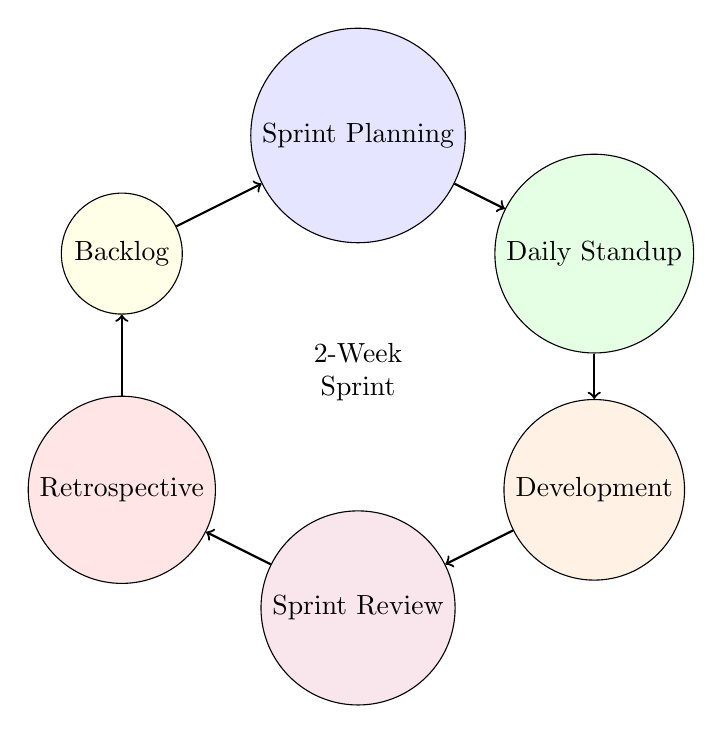
\begin{tikzpicture}
    % Sprint cycle circle
    \node[draw, circle, fill=blue!10, minimum size=1.5cm] (planning) at (0,3) {Sprint Planning};
    \node[draw, circle, fill=green!10, minimum size=1.5cm] (daily) at (3,1.5) {Daily Standup};
    \node[draw, circle, fill=orange!10, minimum size=1.5cm] (development) at (3,-1.5) {Development};
    \node[draw, circle, fill=purple!10, minimum size=1.5cm] (review) at (0,-3) {Sprint Review};
    \node[draw, circle, fill=red!10, minimum size=1.5cm] (retro) at (-3,-1.5) {Retrospective};
    \node[draw, circle, fill=yellow!10, minimum size=1.5cm] (backlog) at (-3,1.5) {Backlog};

    % Arrows showing cycle
    \draw[->, thick] (planning) -- (daily);
    \draw[->, thick] (daily) -- (development);
    \draw[->, thick] (development) -- (review);
    \draw[->, thick] (review) -- (retro);
    \draw[->, thick] (retro) -- (backlog);
    \draw[->, thick] (backlog) -- (planning);

    % Center label
    \node[align=center] at (0,0) {2-Week\\Sprint};

\end{tikzpicture}
\caption{Sprint Cycle: Ahmed's team follows a two-week sprint cadence with regular ceremonies for planning, coordination, review, and continuous improvement.}
\label{fig:sprint-cycle}
\end{figure}


\section{Addressing Change Resistance}
\label{sec:change-resistance}

Not everyone embraced Scrum immediately. Stakeholders accustomed to direct developer requests found the Product Owner intermediary frustrating. Some developers viewed ceremonies as overhead. The organization addressed resistance through demonstrated results. When sprints consistently delivered working software, skeptics recognized the value. Leadership allocated time for ceremonies and protected teams from pressure to bypass process during urgent situations.
